\documentclass[border=4pt]{standalone}
\usepackage{tikz}
\usetikzlibrary{arrows}
\begin{document}
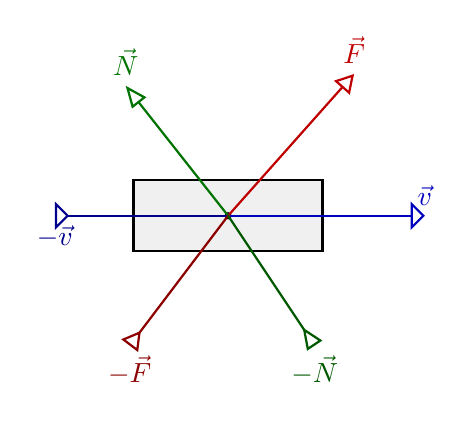
\begin{tikzpicture}[line width=.8pt]
  \draw[fill=gray!12] (-1.2,-.45) rectangle (1.2,.45);
  \fill (0,0) circle (1.3pt);

  \draw[blue!75!black,-{open triangle 90}] (0,0) -- (2.5,0)
    node[above] {$\vec v$};
  \draw[red!75!black,-{open triangle 60}] (0,0) -- (1.6,1.8)
    node[above] {$\vec F$};
  \draw[green!45!black,-{open triangle 45}] (0,0) -- (-1.3,1.65)
    node[above] {$\vec N$};

  \draw[blue!55!black,-{open triangle 90 reversed}] (0,0) -- (-2.2,0)
    node[below] {$-\vec v$};
  \draw[red!55!black,-{open triangle 60 reversed}] (0,0) -- (-1.25,-1.65)
    node[below] {$-\vec F$};
  \draw[green!35!black,-{open triangle 45 reversed}] (0,0) -- (1.1,-1.65)
    node[below] {$-\vec N$};
\end{tikzpicture}
\end{document}
